\documentclass[11pt]{article}
\usepackage[includeheadfoot, top=1.0in, bottom=1.0in, hmargin=1.0in]{geometry}
\usepackage[utf8]{inputenc}
\usepackage{fancyhdr}
\pagestyle{fancy}
\usepackage{setspace}
\usepackage{tabularx}
\usepackage{xcolor}
\usepackage{cancel}
\usepackage{amsmath,amsfonts}
\usepackage{graphicx}
\usepackage{siunitx}
\usepackage{amssymb}

\usepackage{url}
\usepackage{hyperref}

\lhead{Astronomy Lab II}
\rhead{Fall 2024}
\lfoot{Porter}
\rfoot{Wed 6-9pm}
\cfoot{\thepage}

\begin{document}

\begin{center}
\huge{Microsoft Excel Guide}\\ \medskip \Large{Fall 2024}\\ 
\end{center}

%%%%%%%%%%%%%%%%%%%%%%% INTRO %%%%%%%%%%%%%%%%%%%%%%%
Note: this guide was made using a Windows desktop version of Excel. Yours might look different if you're using Excel online or Mac, but the general steps should stay the same. There may be multiple ways to accomplish all of these in Excel, so you may find an alternate method; do what works for you. \\

\textbf{See me if you need help.} \\


\section{How To: Create a Graph}

To create a graph in Excel, ensure you have input all data you want to be graphed into your spreadsheet. Typically, the data going on your x-axis should have one column, while the data going in the y-axis has another column. \\

1. Select data to be graphed. If this is the entire column, select the letters above the column, which automatically grabs the entire column. Hold the "Ctrl" key (Windows) or "Cmd" key (Mac) to select more than one cell/column. \\

2. Go to the toolbar and click "Insert". See Figure~\ref{fig:GraphStep2} \\

3. Find the "Charts" group, and the specific chart you want, such as a scatterplot. Click on the icon. See Figure~\ref{fig:GraphStep3} \\

4. Congratulations! You've made a graph in Excel (see Figure~\ref{fig:GraphStep4}). See below for more details on your graph.

\begin{figure}
    \centering
    
\includegraphics[width=\linewidth]{Images/1step2.png}
    \caption{Step 2 of Create a Graph.}
    \label{fig:GraphStep2}
\end{figure}

\begin{figure}
    \centering
    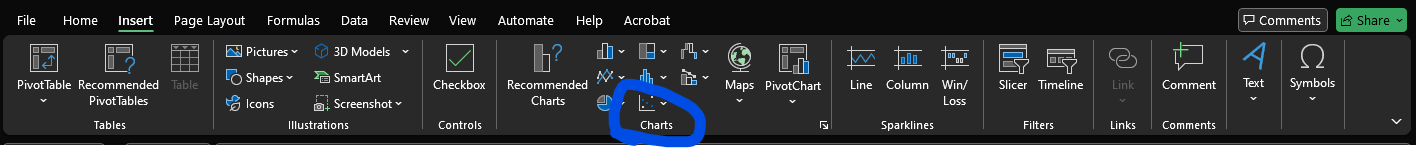
\includegraphics[width=\linewidth]{Images/1step3.png}
    \caption{Step 3 of Create a Graph.}
    \label{fig:GraphStep3}
\end{figure}

\begin{figure}
    \centering
    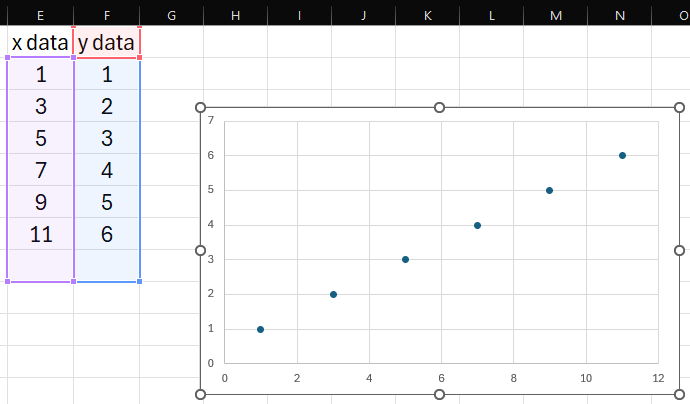
\includegraphics[width=0.75\linewidth]{Images/1step4.png}
    \caption{Completed graph in Excel.}
    \label{fig:GraphStep4}
\end{figure}


\section{How To: Label Your Graphs}

You must have labels on your axes, including units, to get full points! Titles aren't necessary, but nice to have. These steps will be the same for chart titles \emph{and} labelling both axes.

1. Click on your completed graph. \\

2. In the toolbar, go to the "Chart Design" tab, then to the "Chart Layouts" section on the very left. I recommend then clicking "Add Chart Element" so you can pick what you want, but some of the "Quick Layouts", such as the first option, are quicker. See Figure~\ref{fig:Graph2Step2}\\

3. If you didn't select a quick layout,  select the dropdown menu from "Add Chart Element". From here, you can go to "Axis Titles" to add an x- and y-label, or "Chart Title" to give your entire chart a title. \\

4. Your titles and labels can now be edited just like a normal text box: click on the text to change it.

\begin{figure}
    \centering
    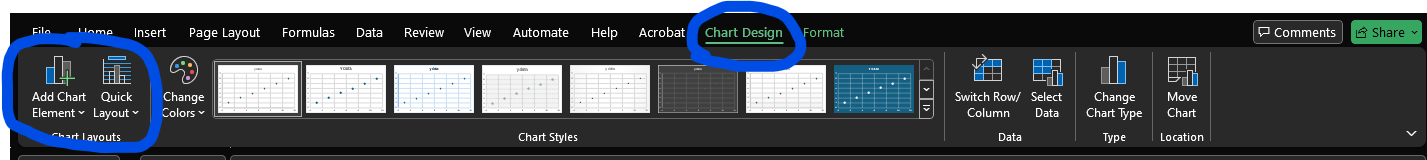
\includegraphics[width=0.75\linewidth]{Images/2step2.png}
    \caption{Step 2 of Label Your Graphs.}
    \label{fig:Graph2Step2}
\end{figure}


\section{How To: Invert Axes}

Inverting, or "flipping" an axis, can be tricky. Here's how to easily do it in Excel without worrying about adjusting your data.

1. Click on your completed graph. \\

2. In the toolbar, go to the "Format" tab. Sometimes this will also appear as "Chart Format"; this is NOT the "Chart Design" tab! Then, find the "Current Selection" box all the way on the left. See Figure~\ref{fig:Graph3Step2}. \\

3. On the dropdown menu, which in Figure~\ref{fig:Graph3Step2} says "Chart Area", click the menu and then the axis you wish to invert: either "Hoizontal (Value) Axis" or "Vertical (Value) Axis". \\

4. On the dropdown menu, which in Figure~\ref{fig:Graph3Step2} says "Chart Area", click the menu and then the axis you wish to invert: either "Hoizontal (Value) Axis" or "Vertical (Value) Axis". Then select "Format Selection", directly below the dropdown menu.

5. You should have had a new window open up on the right side of your screen which looks like Figure~\ref{fig:Graph3Step5}, with "Format Axis" on the top. Make sure you have the fourth image, of the bar chart, selected. The blue arrow in Figure~\ref{fig:Graph3Step5} is pointing to this. \\

6. Find the checkbox with "Values in reverse order", and check that box. This is the underlined box in Figure~\ref{fig:Graph3Step5}. \\

7. Your graph should now be inverted by whichever axis you selected in Step 4. Repeat if you need to invert the other axis.



\begin{figure}
    \centering
    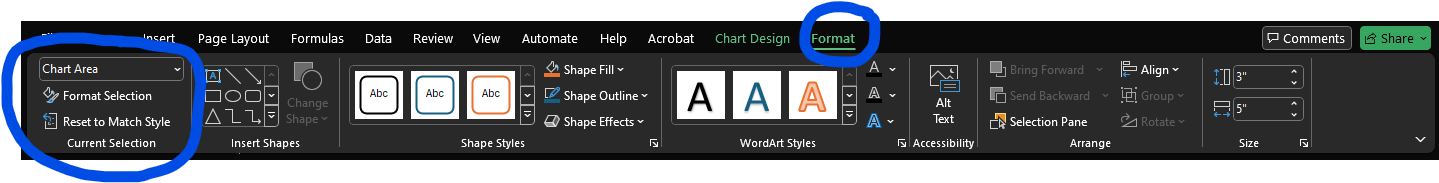
\includegraphics[width=\linewidth]{Images/3step2.png}
    \caption{Step 2 of Invert Axes.}
    \label{fig:Graph3Step2}
\end{figure}

\begin{figure}
    \centering
    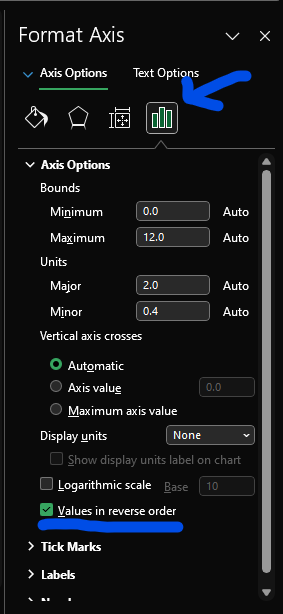
\includegraphics[width=0.3\linewidth]{Images/3step5.png}
    \caption{Step 5 of Invert Axes.}
    \label{fig:Graph3Step5}
\end{figure}


\end{document}
